
%%%%%%%%%%%%%%%
%	Ch6 : Internal Flows	 %
%%%%%%%%%%%%%%%

\chapter{Internal Flows}

\section{Kinematic energy balance (constant density flows)}

Momentum equation: 
\begin{equation}
\rho [\frac{\partial u}{\partial t}+ \vec{u}.\nabla u]=\dot{u}=- \nabla p + \nabla. \bar{\bar{\tau}} + \rho \vec{g}
\end{equation}

To get the kinetic equation, we multiply (scalar porduct) the momentum equation by $\bar{u}$, and by using those assumptions and definitions:

\begin{itemize}
\item Steady flow $\frac{\partial}{\partial t}=0$
\item Body forces derive from a potential $\vec{g}=-\nabla \phi$
\item $k=\frac{\vec{u}.\vec{u}}{2} $
\item $k=\frac{\vec{u}.\dot{\vec{u}}+\vec{u}.\dot{\vec{u}} }{2}= \vec{u}.\dot{\vec{u}} $
\item $\dot{k}=\rho [\underbrace{\frac{\partial k}{\partial t}}_{=0}+\vec{u}.\nabla k]$
\end{itemize}

We get:
\begin{equation}
\rho \vec{u} . \dot{\vec{u}}=\rho \dot{k}= \rho \vec{u}. \nabla k= \rho \nabla . k\vec{u}=\underbrace{- \vec{u}. \nabla p}_{=-\nabla \rho \vec{u}} + 
\underbrace{\vec{u}.  \nabla \bar{\bar{\tau}}}_{u_i \frac{\partial \tau_{ji}}{\partial x_j}}+
 \underbrace{\rho \vec{g} \vec{u}}_{\rho \vec{u}.(-\nabla \phi)=-\rho \nabla \vec{u} \phi}
\end{equation}

Using the continuity equation:
\begin{equation}
\dot{\rho}+\nabla.\rho \vec{u}=0 \ since \  \rho=c^{st} \rightarrow \nabla. \vec{u}=0
\end{equation}

We get:
\begin{equation}
\rho \nabla . k\vec{u}=-\nabla \rho \vec{u}- \rho \nabla \vec{u} \phi+ u_i \frac{\partial \tau_{ji}}{\partial x_j} \Leftrightarrow 
\rho \nabla . k\vec{u}=-\nabla \rho \vec{u}- \rho \nabla \vec{u} \phi+
\underbrace{\frac{\partial }{\partial x_j} (u_i \tau_{ji})}_{\nabla. \vec{u} \bar{\bar{\tau}}}- 
\underbrace{\tau_{ji} \frac{\partial u_i}{\partial x_j}}_{\epsilon_v}
\end{equation}

Where $\epsilon_v=$ viscous dissipation and $\nabla. \vec{u} \bar{\bar{\tau}}=$ power of viscous stresses.

\begin{equation}
\rho \nabla. \vec{u}  \underbrace{[k+\frac{p}{\rho}+\phi]}_{e_m}=\nabla. \vec{u} \bar{\bar{\tau}}-\epsilon_v
\end{equation}

Where $e_m$ = mechanical energy per unit mass. Let's now integrate over a volume V:

\begin{equation}
\rho \int_V\nabla. \vec{u}  [k+\frac{p}{\rho}+\phi]dV=\int_V \nabla. \vec{u} \bar{\bar{\tau}}dV-\int_V\epsilon_v dV
\end{equation}

Let's now apply Gauss theorem:
\begin{equation}
\rho \oint_S[k+\frac{p}{\rho}+\phi]  \vec{u}.\vec{n}  dS=\oint_S  \vec{u}. (\bar{\bar{\tau}}.\vec{n}) dS- \underbrace{\int_V\epsilon_v dV}_{>0}
\end{equation}

There is no mass flow through the walls of the pipe, the only contributions are then the ones from the inlet(1) and outlet(2) sections.

Normal viscours stresses on the inlet and outlet can be considered negligeable, for high Reynolds number, if the pipe is long enough, such that the surface intgrals have a smaller contribution than the viscous dissipation:

\begin{equation}
\oint_S  \vec{u}. (\bar{\bar{\tau}}.\vec{n}) dS=0 \Leftrightarrow  
\int_2  \bar{\tau}^{(\vec{n})}.\vec{u} dS-\int_1  \bar{\tau}^{(-\vec{n})}.\vec{u} dS=0
\end{equation}

So we have:

\begin{equation}
\rho \int_2[k+\frac{p}{\rho}+\phi]  \vec{u}.\vec{n}  dS
+\rho \int_1[k+\frac{p}{\rho}+\phi]  \vec{u}.(-\vec{n})  dS
=- \int_V\epsilon_v dV
\end{equation}

Since $k=\frac{\vec{u}^2}{2}$ and $\phi=gz$, and by introducing the notation for the average of a quantity:  $average \ of \  x=<x>$, we get:

\begin{equation}
<\frac{\vec{u}^2}{2}+\frac{p}{\rho}+gz>_{2,1} \equiv \frac{\rho \int[\frac{\vec{u}^2}{2}+\frac{p}{\rho}+gz]  \vec{u}.\vec{n}  dS}{\dot{m}}
\end{equation}

By using this definition, the last expression of the kinetic equation that we have obtained becomes:

\begin{equation}
<\frac{\vec{u}^2}{2}+\frac{p}{\rho}+gz>_{2} - <\frac{\vec{u}^2}{2}+\frac{p}{\rho}+gz>_{1}=-\frac{ \int_V \epsilon_v dV }{\dot{m}} \equiv -e_f
\end{equation}

Where $e_f=$ viscous losses per unit mass $[\frac{J}{kg}] \Leftrightarrow [{\frac{m}{s}}^2]$

Assuming the flow is purely normal (no cross flow), then the average velocity can be defined as:

\begin{equation}
<u>=\frac{\int \rho u dS}{\int \rho dS}=\frac{\int  u dS}{S} (\ because \ \rho=c^{st})
\end{equation}

In most cases $p=c^{st} and \phi=c^{st}$ (p and $\phi$ uniform across section). We these assumptions we can now find the average value for $h=\frac{u^2}{2}$, $\frac{p}{\rho}$ and $gz$.

\begin{equation}
<k>=<\frac{u^2}{2}>=\frac{\rho \int_S \frac{\vec{u}^2}{2} \vec{u}.\vec{n}  dS} {\rho \int_S  \vec{u}.\vec{n}  dS} \ (by \ definition)
\end{equation}

By using the definition of $<u>$, we get:

\begin{equation}
<k>=<\frac{u^2}{2}>=\frac{\int_S \frac{\vec{u}^2}{2} \vec{u}dS} {<u>S}=\frac{<u>^2}{2} \frac{1}{S} 
\underbrace{\int_S (\frac{u}{<u>})^3 dS}_{=\alpha}
\end{equation}

\begin{equation}
<k>=\alpha \frac{<u>^2}{2}
\end{equation}

Where $\alpha$ is the kinetic energy factor (also called non dimensionnal shape factor).
\begin{itemize}
\item For uniform flow $\alpha=1$
\item For parabolic laminar Poiseuille flow $\alpha=2$
\item For turbulent flow $1.04<\alpha<1.1$
\end{itemize}

Since  $p=c^{st} and \phi=c^{st}$ the average value is found easily:
\begin{itemize}
\item $<\frac{p}{\rho}>=\frac{<p>}{\rho}$
\item $<gz>=g<z>$
\end{itemize}

By putting everything together we get:
\begin{equation}
[\alpha \frac{<u>^2}{2}+\frac{<p>}{\rho}+g<z>]_{inlet}^{outlet}=-e_f
\end{equation}


\section{Distributed losses (Major losses) for a fully developped flow in a (circular) cylinder}

Main assumptions:
\begin{itemize}
\item Fully developped flow: A fully developped/established flow does not vary across the pipe's length: $U_{inlet(1)}=U_{outlet(2)}$.
\item Constant density flow
\item Constant section
\end{itemize}

Mass conservation: $\dot{m_1}=\dot{m_2} \Leftrightarrow \rho_1 U_1S_1=\rho_2 U_2S_2$ by applying our asumptions we get: $\rho US=c^{st}$ 

Axial momentum balance: net axial momentum flow out= sum of the forces. By taking into account our assumptions we see that there is no net mass flow out. And so the axial momentum balance is resumed to: sum of the forces equals zero.

\begin{equation}
Sum \ of \ the \ forces=0 \Leftrightarrow -\rho SL cos \theta g+ p_1 S-p_2 S- \tau_w P_{er} L=0
\end{equation}
\begin{equation}
\Leftrightarrow  -\rho S(z_2-z_1) g+ p_1 S-p_2 S- \tau_w P_{er} L=0
\end{equation}
\begin{equation}
\Leftrightarrow  -\rho S[\frac{p_2}{\rho}+gz_2-(\frac{p_1}{\rho}+gz_1)]=-\tau_w P_{er} L
\end{equation}
\begin{equation}
\Leftrightarrow [\frac{p}{\rho}+gz]_1^2=\frac{-\tau_w P_{er} L}{\rho S }
\end{equation}

By comparing this result with the kinetic equation for a fully developped flow, we get:
\begin{equation}
e_f=\frac{\tau_w P_{er} L}{\rho S }
\end{equation}
By multiplying this equation by $\frac{4D_h}{4D_h}$ where $D_h$ is the hydraulic diameter and is defined by $D_h=\frac{4S}{P_{er}}$, we get:

\begin{equation}
e_f=\frac{\tau_w}{\rho} 4D_h \frac{P_{er}}{4S}\frac{L}{D_h} \ (for \ a \ circular \ pipe \ D_h=\frac{4 \pi D^2/4}{\pi D}=D)
\end{equation}
\begin{equation}
\Leftrightarrow e_f=\frac{4 \tau_w}{\rho} \frac{L}{D_h}
\end{equation}

We can define a new quantity $f$ which is called the Darcy-Weisbach friction factor (Noted $\lambda$ in French and called "coefficient de perte de charge"):
\begin{equation}
f=\frac{e_f}{\frac{L}{D_h}}\frac{2}{\rho <u>^2}
\end{equation}

Remembering that $C_f=\frac{2 \tau_w}{\rho <u>^2}$, we see that:
\begin{equation}
f=4C_f
\end{equation}

\textbf{Dimensionnal analysis:} To perform dimensionnal analysis we have to imagine on which variables the quantity will depend.
Note: Loss is proportionnal to the pipe's length: $e_f \propto L$. Let's do it:
\begin{equation}
\frac{e_f}{\frac{L}{D_h}}=(\frac{4 \tau_w}{\rho})=g(<u>, \nu, D_h, \underbrace{\epsilon}_{roughness \ heigth})
\end{equation}

We have 5 quantities and 2 physical dimensions, by applying Buckingham's $\Pi$ Theorem, we have to find 3 dimensionless groups:
\begin{equation}
\underbrace{\frac{e_f}{\frac{L}{D_h} \frac{<u>^2}{2}}}_{1^{st}group}=\Psi(\underbrace{\frac{<u>D_h}{\nu}}_{2^{nd}group},\underbrace{\frac{\epsilon}{D_h}}_{3^{d}group})
\end{equation}

From this point on, Pr. Degrez mostly uses the slides from Pr. Coussement (from Mons university) and completes them with somes notes on the blackboard. Here follows a resume of the important things pointed in those slides during the course by Pr. Degrez.
\\

For the ones interested to go back to those slides instead of this resume, the chapter to consult is the chapter (page 208 to 261): "XX. Introduction au transport de fluides par canalisations". You can skip the section "XX.f. Cavitation" as Pr. Degrez did.
\\

For simplicity, since those slides are in French, I will continue in French.

\selectlanguage{french}
\section{Introduction au transport de fluides par canalisations (Cours de Mons)}

Ce chapitre reprend les développements fait ci-dessus. Je note donc ici uniquement les éléments nouveaux ainsi que les remarques et observations interessantes.\\

\textbf{Definitions:}
\begin{itemize}
\item Pertes de charges régulières (réparties): pertes d'énergie mécanique dans les tronçons rectilignes à section constante.
\item Pertes de charges singulières (locales): pertes d'énergie mécanique dans les autres parties (sauf systèmes récepteurs ou générateurs).
\end{itemize}

Notes: 
\begin{itemize}
\item L'equation de continuité: $\rho US=c^{st}$ montre que si la section diminue, la vitesse augmente (et vice versa).
\item On peut démontrer que, si les filets fluides sont parallèles et de faible courbure, la répartition de pression dans une section normale obeit à la loi hydrostatique: $\frac{p}{\rho}+gz=c^{st}$ dans une section.
\item $\alpha$= coefficient de forme tenant compte de la non-uniformité du profil de vitesse dans la section S. La valeur de $\alpha$ dépend du type de section et du type d'écoulement. Les valeurs de $\alpha$ pour différents profils de vitesses sont représentés à la figure 6.1. Remarque: En écoulement turbulant, la loi de vitesse est de type "loi de puissance" sauf dans le voisinage de la paroi (sous-couche laminaire). 
\begin{figure}[h]
\begin {center}
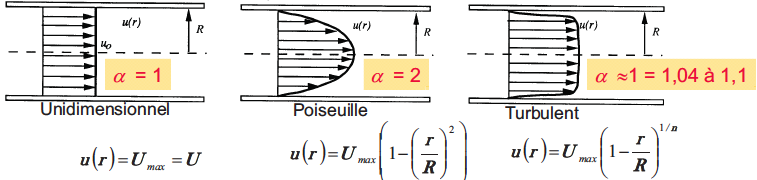
\includegraphics[scale=0.35]{ch6/61.png}
\caption*{Figure 6.1}
\end{center}
\end{figure}
\item En fluide parfait, il y conservation du débit d'energie totale, alors qu'en fluide visqueux il y a une dégradation de l'énergie dans le sens de l'écoulement. Cette dégradation d'énergie (=perte de charge) se note $\tau_w$ et correspond à la perte d'énergie mécanique due aux frottements visqeux dans la canalisation.
\item La puissance nécessaire pour transporter le fluide d'un bout du tronçon (A) à un autre (B) = la puissance nécessaire pour combattre les pertes par frottements entre A et B= la puissance dissipée par les perte de charges entre A et B.
\item Un récapitulatif est repris sur la figure 6.2.
\end{itemize}

\begin{figure}[h]
\begin{center}
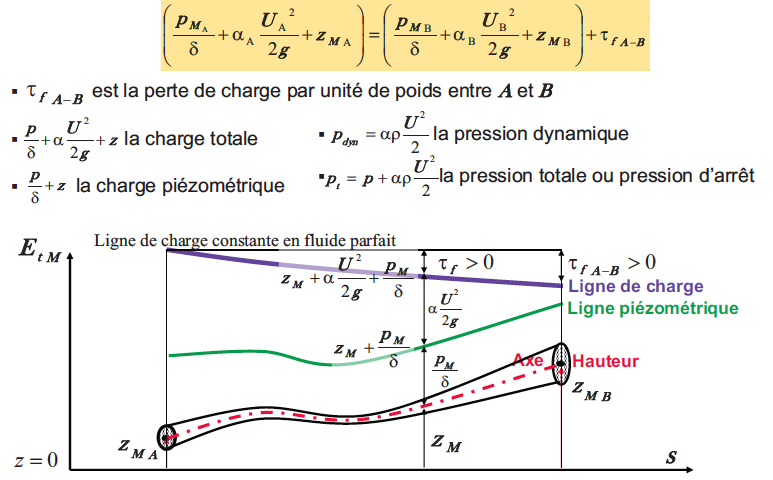
\includegraphics[scale=0.45]{ch6/62.png}
\caption*{Figure 6.2}
\end{center}
\end{figure}

\section{Pertes de charges réparties (Cours de Mons)}

En premier lieu on considère une conduite cylindrique longue et à section circulaire. Voici les hypothèses qui sont faites pour cette partie:
\begin{itemize}
\item Axe rectiligne
\item Section circulaire constante
\item Pas d'éléments perturbateurs (vannes, coudes, ...)
\item Canalisation suffisament longue pour considérer l'écoulement comme établi (c.à.d. profil de vitesse identique d'une section à l'autre). Cette hypothèse implique $\alpha=c^{st}$
\item Ecoulement permanent
\item Ecoulement incompréssible
\item Ecoulement soumis aux forces de pesanteur \\
\end{itemize}


\textbf{Analyse de la rugosité:} (vu dans la section 4.3.1. "Inner zone (rough wall)") du cours du Pr. Degrez.

La rugosité, qui est le facteur essentiel de la paroi, influence nettement les dégradations énergétiques. La rugosité dépend de: 
\begin{itemize}
\item La hauteur moyenne des aspérités
\item Des variations de hauteur par rapport à la hauteur moyenne
\item De la forme et de la répartition des aspérités
\end{itemize}
L'effet de la rugosité sur les pertes se fait via des relations semi-empiriques. Une déscritption mathématique étant trop compliquée.
\\

Une première analyse des efforts sur les tronçons d'une tuyauterie indique que la perte de charge $(\tau_f)$ est proportionnelle à la longueur relative $(L/D)$ du tronçon et au frottement $(\tau_p)$ à la paroi. Pour déterminer  $(\tau_f)$ , il faut déterminer $(\tau_p)$. Ce dernier ne peut être déterminé analytiquement. On utilise donc l'analyse dimensionnelle ainsi que l'expérience pour le déterminer.
\\
Cette analyse dimensionnelle a été faite au 6.2. Celle faite dans ces slides est faite de manière beaucoup plus détaillée mais le résultat est le même (Attention il s'agit ici des notations françaises et non anglaises!). Je la reprend ici dans les grandes lignes. 

L'analyse dimensionnelle permet de determiner le nombre d'essais minimum à réaliser en fonction des différents paramètres pour pouvoir à l'aide de l'experimentation déduire des relations empiriques générales. L'analyse dimensionnelle est faite ici en utilisant le théorème des $\Pi$:

\begin{enumerate}
\item De quelles quantités dépend $(\tau_f)$ ?  $\tau_f=f(U,D,\rho,\mu, L, \epsilon,g)$
\item 8 quantités et 3 dimensions, on doit donc déterminer 5 groupes adimensionnels
\item On trouve: $\frac{(\tau_f)}{\frac{U^2}{2g}}=f(\frac{L}{D},\frac{\epsilon}{D},Re,Fr)$
\\
\end{enumerate}

Comme on l'a vu dans le cours, le nombre de Froude est négligeable (pou rappel le nombre de Froude traduit l'influence de  $g$):
\begin{itemize}
\item Pour les gaz, la masse spécifique est faible, l'influence de $g$ est négligeable
\item On a vu, que le nombre de Froude n'a d'influence que dans le cas des surfaces libres
\\
\end{itemize}

On introduit ici le coefficient de perte de charge $\lambda$ (f en anglais). Ses dépendances sont: $\lambda=f(Re,\frac{\epsilon}{D})$. L'expression de $\tau_f$ devient alors:  $\tau_f=\lambda \frac{U^2}{2g} \frac{L}{D}$. Le calcul del a perte de charge ($\tau_f$) revient donc à déterminer la fonction qui donne la valeur du coefficient de perte de charge $\lambda$.
\\

Comme on l'a vu, le coefficient de perte de charge $\lambda$ est directement proportionnel au coefficient de frottement $C_f$. En effet on a: $\lambda=4C_f$.

Etudions maintenant les effets des conduites lisses $(\epsilon/D=0)$, rugeuses homogènes et rugeuses hétérogènes.
\\

\textbf{Conduites lisses:} \\
\begin{wrapfigure}[9]{l}{6.5cm}
\vspace{-5mm}
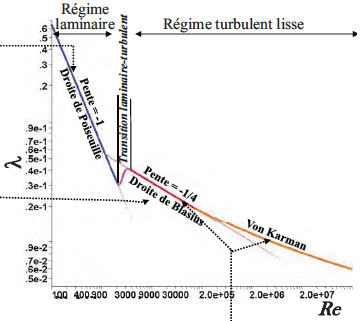
\includegraphics[scale=0.50]{ch6/64.png}
\caption*{Figure 6.3}
\end{wrapfigure}
Pour l'écoulement laminaire de Poiseuille on trouve: $\lambda=\frac{64}{Re}$ ou encore $log\lambda=log64-logRe$ qui est la droite de Poiseuille. L'expérience montre que cette droite est respectée pour Re allant jusqu'à $2000-3000$. Pour $2000<Re<4000$ on a une zone de transition. Au delà, l'écoulement devient turbulent. En pratique, l'écoulement est toujours turbulent à partir de $Re=10000$.
\\
Deux zones de turbulences peuvent être distinguées:
\begin{itemize}
\item La zone où $4000<Re<100000$ dans laquelle on peut utiliser la droite de Blasius: $log\lambda=log0,3164-\frac{1}{4}logRe$.
\item La zone où $Re>100000$ dans laquelle on peut utiliser la règle généralisée de Von Karman ou Prandt-Nikuradse: $\frac{1}{\sqrt{\lambda}}=-2log\frac{2,51}{Re\sqrt{\lambda}}$. Cette droite peut être utilisée à partir de $Re>4000$. Son écart avec la droite de Blasius est négligeable.\\
\end{itemize}

\textbf{Conduites aux rugosités homogènes:} 
\\
On constate premièrement que la rugosité n'influence pas le comportement de $\lambda$ dans la zone laminaire. Par contre lorsque le nombre de Reynolds augmente, l'écoulement devient turbulent et:
\begin{itemize}
\item Pour $Re < Re_1$, comme dans le cas d’une conduite
lisse, les points expérimentaux se déplacent sur la même courbe de transition puis sur la même droite de
Blasius : Le régime est dit «hydrauliquement lisse» et
$\lambda=f(Re)$ uniquement.
\item Au delà d’un $Re_1$ critique dépendant de $\epsilon/D$, les points expérimentaux ne suivent plus la même évolution que celle d’une conduite lisse. Il y a une incurvation vers le haut de la courbe puis à partir d’un second $Re_2$ critique $(Re>Re_2)$, la valeur de $\lambda$ ne varie plus avec Re : $\lambda=f(\epsilon/D)$ uniquement (Zone « hydrauliquement rugueuse »). Dans cette zone, $\lambda$ est donné par la loi de Prandtl-Karman: $\frac{1}{\sqrt{\lambda}}=-2log(\frac{\epsilon}{3,71D})$
\\
\end{itemize}

La figure ci-dessous reprend ces différentes zones:
\begin{figure}[h]
\begin{center}
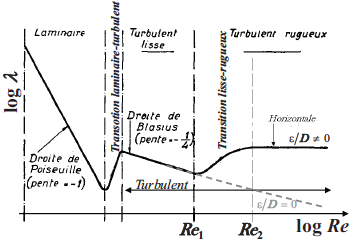
\includegraphics[scale=0.50]{ch6/65.png}
\caption*{Figure 6.4}
\end{center}
\end{figure}

\textbf{Conduites aux rugosités hétérogènes:} 
\\
La figure ci-dessous reprend l'essentiel du cas des conduites aux rugosités hétérogènes et montre également les différences avec le cas des conduites aux rugosités homogènes. La différence la plus importante à remarquer c'est le passage par un minimum dans le cas homogène qui ne se trouve pas dans le cas hétérogène.
\\

\begin{figure}[h]
\begin{center}
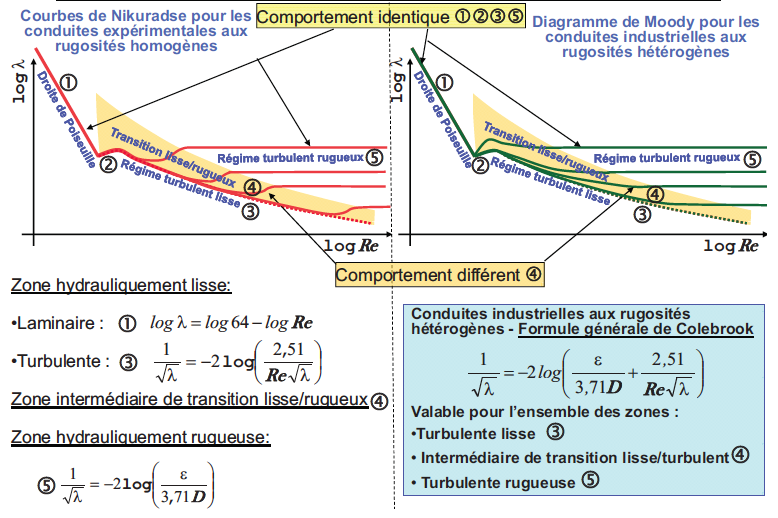
\includegraphics[scale=0.4]{ch6/66.png}
\caption*{Figure 6.5}
\end{center}
\end{figure}

Remarque: La rugosité $\epsilon$ des conduites industrielles aux rugosités hétérogènes est un paramètre d'équivalence et n'est pas nécessairement la représentation de la hauteur moyenne des aspérités réelles. Dans la zone quadratique (=zone hydrauliquement rugueuse), $\epsilon$ est identique au $\epsilon$ homogène qui donne un $\lambda$ identique au $\lambda$ mesuré avec le $\epsilon$ hétérogène. On se reporte à des catalogues pour déterminer cette rugosité. Le diagramme de Moody ($\lambda$ en fonction de $Re$) est le diagramme de l'évolution de $\lambda$ pour des conduites industrielles à rugosité hétérogènes.
\\

\textbf{Analyse de l'influence de la rugosité sur la distribution des vitesses} 
\\
Comme vu au cours (section 4.3.1 du cours du Pr. Degrez), on a un régime lisse si les rugosités sont dans la sous-couche laminaire.
\\

Note: Pour les rugosités homogène (ayant toutes la même hauteur), avec $Re \uparrow$ ou $\epsilon \uparrow$, comme les rugosités atteingent toutes simultanément la zone de transition laminaire/turbulant puis la zone de turbulence pleinement, la transition du régime lisse vers le régime turbulent rugueux est relativement brutale. Au contraire, pour les rugosités hétérogènes, cette transition est plus progressive étant donnés que les rugosités, ayant des hauteurs différentes, celles-ci sont parfois dans la sous-couche visqueuse laminaire, la zone de transition ou la zone de turbulence.
\\

Les figures ci-dessous reprennent les informations importantes concernant l'influence de la rugosité sur le profil des vitesses.

\begin{minipage}{0.49\textwidth}
\begin{figure}[H]
\begin{center}
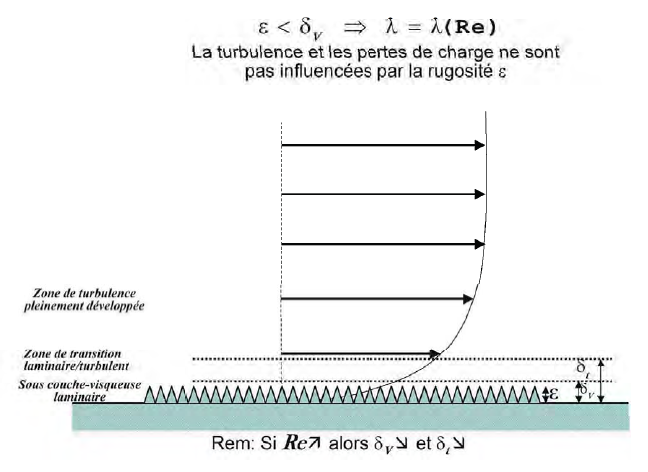
\includegraphics[scale=0.35]{ch6/67.png}
\caption*{Figure 6.6}
\end{center}
\end{figure}
\end{minipage}
\begin{minipage}{0.49\textwidth}
\begin{figure}[H]
\begin{center}
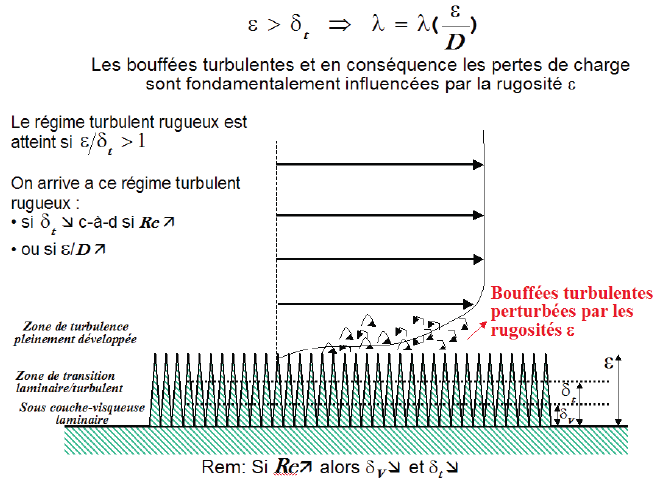
\includegraphics[scale=0.35]{ch6/68.png}
\caption*{Figure 6.7}
\end{center}
\end{figure}
\end{minipage}

\begin{figure}[H]
\begin{center}
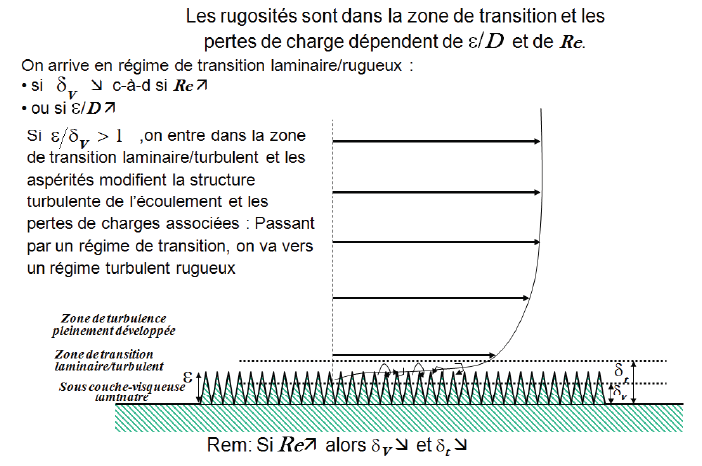
\includegraphics[scale=0.40]{ch6/69.png}
\caption*{Figure 6.8}
\end{center}
\end{figure}


Cas des conduites non-circulaires:  On revient à des relations similaire au cas d'une canalisation en définissant un diamètre hydraulique \og  équivalent\fg{} noté $D_h$.
\begin{itemize}
\item Rayon hydraulique est défini par: $R_h=\frac{S}{P_{er}}$ où $S$= l'aire de la section et $P_{er}$= le périmètre.
\item Le diamètre hydraulique est défini par: $D_h=4R_h=\frac{4S}{P_{er}}$
\end{itemize}

\section{Pertes de charges singulières/locales (Cours de Mons)}

La figure 6.9 reprend les différents types de singularités que l'on peut rencontrer.

Remarque: Les pompes et les turbines ne sont pas des singularités. Il fournissent (pompes) ou retirent (turbines) de l'énergie mécanique au fluide par l'interaction du fluide avec des pièces mécaniques en mouvement.
\\

\begin{figure}[h]
\begin{center}
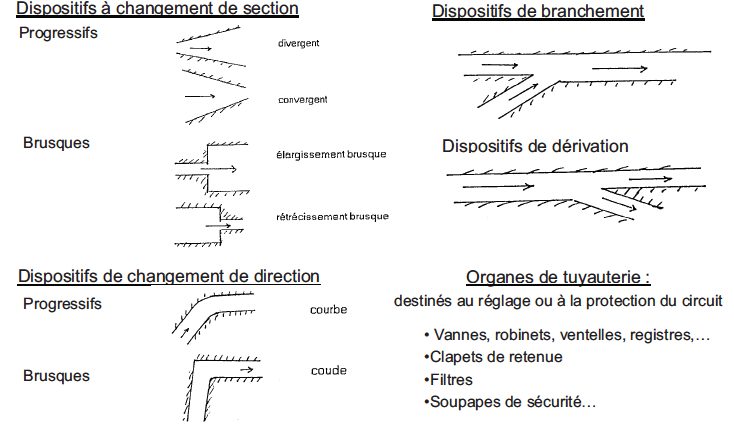
\includegraphics[scale=0.45]{ch6/70.png}
\caption*{Figure 6.9}
\end{center}
\end{figure}

La perte de charge locale $\tau_{floc}$ mesure, par rapport aux pertes régulières, l’énergie mécanique supplémentaire perdue par le fluide lors de son passage dans la singularité. Cette perte de charge locale s’obtient en prolongeant les parties droites de la perte de charge répartie jusqu'aux sections d'entrée A et de sortie B de la singularité. La perte de charge locale est alors donnée par l'écart : $\tau_{floc}=E_{tfA}-E_{tfB}$ où  $E_{tfA} \ et \ E_{tfB}$ représentent les énergies totales fictives (charges totales fictives) à l’entrée A et de sortie B obtenue en ne considérant que les pertes
de charge réparties à l’amont de A et à l’aval de B. Cette définition revient donc à concentrer l’effet de perte supplémentaire due à la singularité entre l’entrée A et la sortie B de la singularité (cf. figure 6.10).

\begin{minipage}{0.49\textwidth}
\begin{figure}[H]
\begin{center}
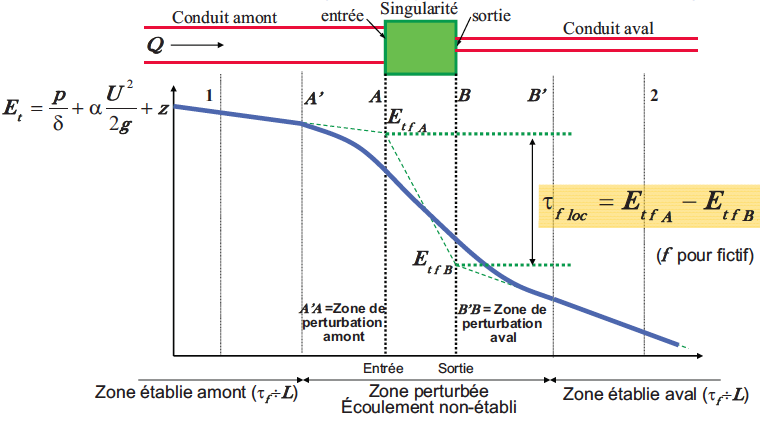
\includegraphics[scale=0.3]{ch6/71.png}
\caption*{Figure 6.10}
\end{center}
\end{figure}
\end{minipage}
\begin{minipage}{0.49\textwidth}
\begin{figure}[H]
\begin{center}
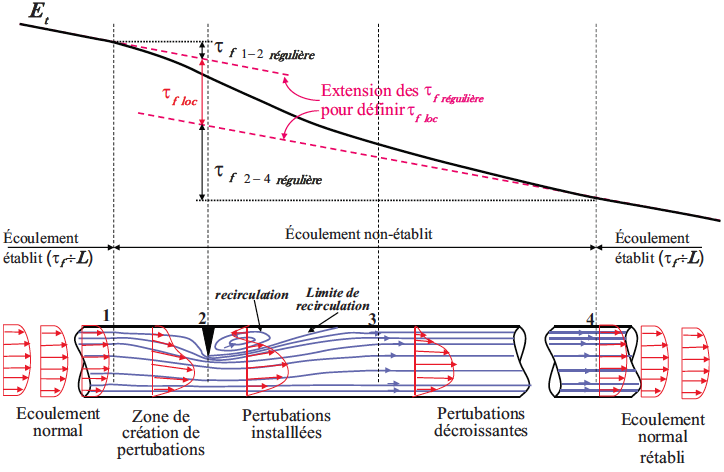
\includegraphics[scale=0.25]{ch6/72.png}
\caption*{Figure 6.11}
\end{center}
\end{figure}
\end{minipage}

Une analyse dimensionnelle permet cette fois-ci de trouver l'expression de la perte de charge locale. On trouve: $\tau_{floc}=\zeta \frac{U^2}{2g}$ où $\zeta=f$(Re, type de singularité, nature de la paroi et son état de surface).  $\zeta$ est le coefficient sans dimensions de perte de charge local (notée $K_L$ en anglais et appelé \og minor loss coefficient \fg{}).
\\

Note: Par convention, on prend Re,D et U correspondant à la plus petite section.
\pagebreak 

La figure 6.12 illustre l'évolution du coefficient de perte de charge locale en fonction du nombre de Reynolds. On y observe que:
\begin{itemize}
\item Au dessus d’un certain Reynolds critique $Re^*$, le régime est turbulent rugueux et ne dépend plus du Reynolds. De plus, pour la majorité des singularités,  $\zeta$ dépend peu de la rugosité mais dépend essentiellement de la géométrie de la singularité. Pour un singularité donné $\zeta$ est donc constant ($\zeta=c^{st}$).
\item Au contraire pour des petits Reynolds ($Re<2000$), le régime est laminaire et $\zeta \propto 1/Re$
\end{itemize}.

\begin{figure}[H]
\begin{center}
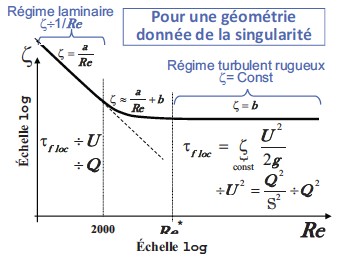
\includegraphics[scale=0.5]{ch6/73.png}
\caption*{Figure 6.12}
\end{center}
\end{figure}

\textbf{Analyse de la perte de charge locale dans les convergents progressifs et brusques:}

Le plus important à comprendre dans le cas d'un convergent progressif c'est que comme la vitesse augmente (car surface diminue), la pression diminue (la pression à l'entrée est plus élevée que celle à la sortie). La pression à donc pour effet de \og pousser \fg{} le fluide dans le sens de l'écoulement. Ceci à pour conséquence d'éviter le décollement. La perte de charge est négligeable pour un convergent progressif.

Dans le cas d'un convergent brusque par contre, la perte de charge n'est pas négligeable. On observe les phénomènes de séparation et recirculation dans la couche limite. Il y a des décollements de la couche limite et des écoulements tourbillonaires sont induits par ces décollements.

Le cas d'un convergent progressif est repris dans la figure 6.13. 

\begin{figure}[h]
\begin{center}
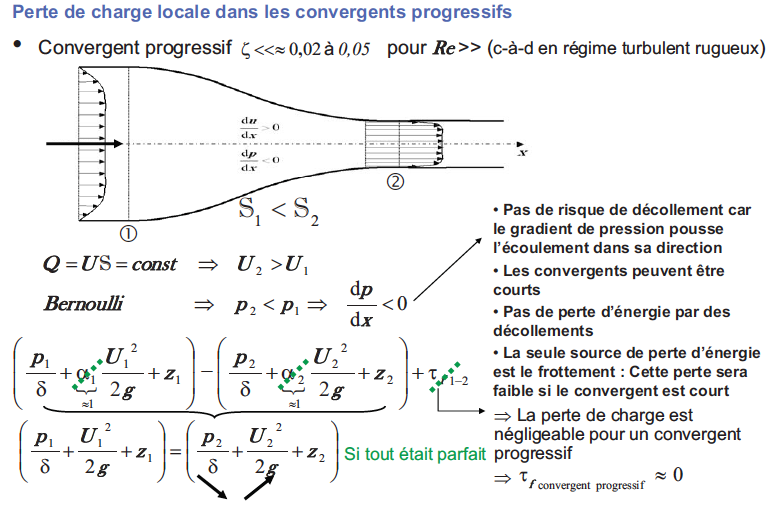
\includegraphics[scale=0.40]{ch6/74.png}
\caption*{Figure 6.13}
\end{center}
\end{figure}

\textbf{Analyse de la perte de charge locale dans les divergents progressifs et brusques:}

Dans ce cas ci, la vitesse diminue et donc la pression augmente. Le gradient de pression s'oppose donc à l'écoulement ce qui aura un effet néfaste.

Pour un petit angle d’ouverture, l’écoulement se ralentit suite à l’augmentation de la section (cons. masse)
et en conséquence la pression augmente (Bernoulli) créant un « gradient adverse de pression » Avec un angle d’ouverture plus grand, le gradient adverse de pression s’intensifie: si l’énergie cinétique des zones à basse vitesse située près des parois n’est plus suffisante pour s’opposer au gradient adverse de la pression, il y a inversion des vitesses et décollement (écoulement de retour) avec une zone de recirculation. Dans cette zone tourbillonnaire de recirculation, les pertes par frottement sont fortes et la perte de charge est donc importante.

Le cas d'un divergent progressif est repris dans la figure 6.14. 

\begin{figure}[H]
\begin{center}
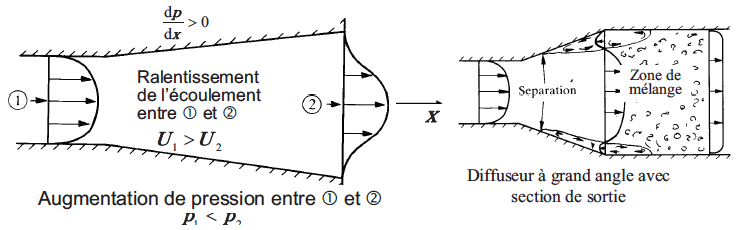
\includegraphics[scale=0.40]{ch6/75.png}
\caption*{Figure 6.14}
\end{center}
\end{figure}

On observe que l'angle maximum $2\theta$ avant décollement pour un diffuseur conique est de l'ordre de $7\deg$. Cet angle correspond à l'angle donnant une perte de charge minimum au diffuseur. On peut expliquer ce minimum comme suit: 

\begin{itemize}
\item Si l’angle d’ouverture est très petit, le gradient adverse de pression dû à l’élargissement est très faible,
l’énergie cinétique se transforme lentement en énergie de pression, sans trop de pertes, mais il faut une
grande longueur de diffuseur pour passer de la section $S_1$ à la section $S_2$. La perte de charge est alors surtout due aux frottements sur les parois, comme pour une conduite cylindrique longue.
\item Lorsque l’angle d’ouverture est inférieur à $7\deg$, les vitesses lorsque l’on se rapproche des parois se ralentissent plus vite que celles de la zone centrale sous l’effet du gradient adverse de pression. Le profil de vitesse tend vers un profil ayant un point d’inflexion sans pour autant atteindre le décollement. La tension à la paroi $\tau_p=\mu \frac{\partial u}{\partial y}$ diminue pour tendre vers 0 si le profil de vitesse présente un point d’inflexion à la paroi. La tension à la paroi diminuant, les pertes par fortement diminuent et atteignent un minimum pour un angle $2\theta$ de $7\deg$.
\item Si l’angle d’ouverture est assez grand, le diffuseur est court, les pertes par frottement sont réduites, mais les pertes par mélange sont fortes. En effet, dans une section perpendiculaire à l’axe, la répartition des vitesses présente un maximum accentué au centre. Quand l’angle d’ouverture dépasse $2\theta=7\deg$, le fluide fini par décoller des parois, ce qui n’est pas favorable à la conservation de l’énergie mécanique : la recirculation dans la zone décollée créant des pertes tourbillonnaires importantes. A partir de
$2\theta>7\deg$, la perte de charge locale se met à augmenter (cf. figure 6.15).
\item Si le divergent est trop ouvert, le décollement apparaît dès le début du divergent. Il se forme un jet qui peut se plaquer contre l’une des parois ou qui oscille entre les parois. La perte de charge est importante et est alors analogue à celle qui se produit dans un élargissement brusque.
\end{itemize}

\begin{figure}[H]
\begin{center}
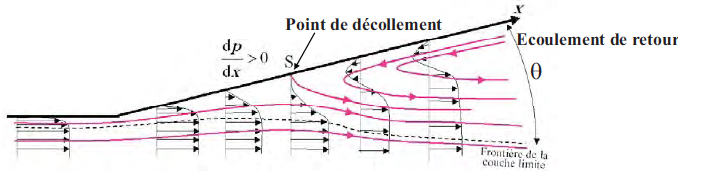
\includegraphics[scale=0.40]{ch6/76.png}
\caption*{Figure 6.15}
\end{center}
\end{figure}

\textbf{Contrôle intermédiaire de l’angle de diffusion par soufflets (système passif):}

Pour un n soufflets, entre deux soufflets, l’angle d’ouverture diminue et vaut $2 \theta /n$. Si $2 \theta /n$ est suffisamment faible, les décollements disparaissent et les pertes associées à ces décollements disparaissent. Cependant, il existe un compromis entre un nombre suffisant de soufflets pour supprimer les pertes par décollement et pas trop grand pour limiter les pertes par frottement sur les parois supplémentaires des soufflets (cf. figure 6.16).

\begin{figure}[H]
\begin{center}
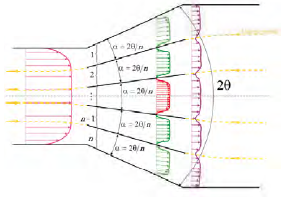
\includegraphics[scale=0.50]{ch6/77.png}
\caption*{Figure 6.16}
\end{center}
\end{figure}

\textbf{Contrôle du développement et du décollement de la couche limite par aspiration ou soufflage de la zone déficitaire (système actif):}

\begin{itemize}
\item Contrôle par aspiration de la zone déficitaire : Suppression de la zone déficitaire en énergie cinétique dans la zone située près de la paroi. Ceci empêche le décollement et limite donc les pertes dues au décollement.
\begin{figure}[H]
\begin{center}
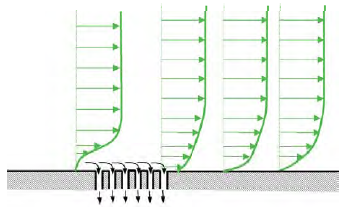
\includegraphics[scale=0.40]{ch6/78.png}
\caption*{Figure 6.17}
\end{center}
\end{figure}
\item Contrôle par soufflage de la zone déficitaire : Augmentation de l’énergie de la zone déficitaire en énergie cinétique située près de la paroi. Ceci empêche le décollement et limite donc les pertes dues au décollement.
\begin{figure}[H]
\begin{center}
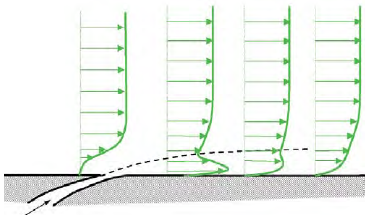
\includegraphics[scale=0.40]{ch6/79.png}
\caption*{Figure 6.18}
\end{center}
\end{figure}
\end{itemize}

\textbf{Pertes de charges dans les coudes:}

En fonction de l’angle du coude et du rayon de raccordement, des décollements apparaîtront au niveau de l’intérieur (Zone 1) et de l’extérieur (Zone 2) du coude (cf. figure 6.19).

\begin{figure}[H]
\begin{center}
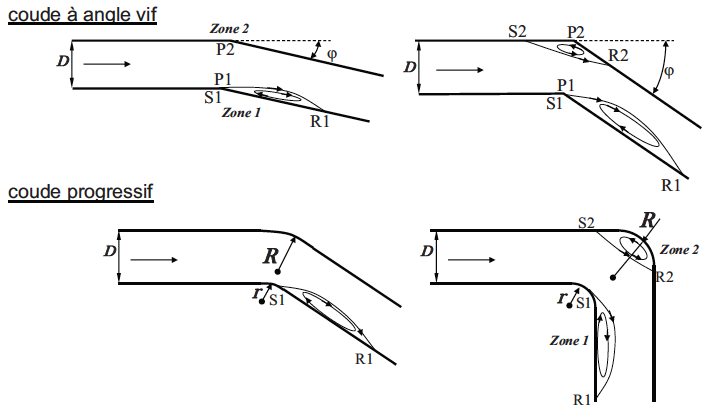
\includegraphics[scale=0.40]{ch6/80.png}
\\
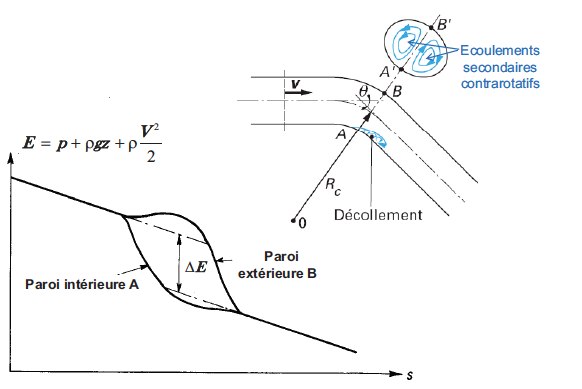
\includegraphics[scale=0.40]{ch6/81.png}
\caption*{Figure 6.19}
\end{center}
\end{figure}

Si on se déplace de B vers A en restant toujours au voisinage de la paroi, on est dans la zone à vitesse faible de la couche limite : l’énergie cinétique y est faible. La différence de pression entre B et A poussera préférentiellement ces particules proches de la paroi à faible énergie cinétique plutôt que celles situées au centre qui ont une énergie cinétique importante et qui seront donc moins facilement déviées.

$\rightarrow$ Dans une section transversale, sous l’effet du gradient de pression existant entre B et A ($P_B > P_A$), les particules fluides à faible énergie cinétique situées le long de la paroi se déplaceront de B vers A le long de la paroi.

$\rightarrow$ Le débit devant se conserver, il en résulte l’apparition d’un écoulement en sens inverse (de A vers B) au centre de la section transversale. Ceci crée 2 recirculations secondaires sous forme de tourbillons contrarotatifs dans la section transversale. Ces 2 tourbillons secondaires sont le lieu d’une dissipation d’énergie causant des pertes de charge supplémentaires : Ces 2 tourbillons secondaires retirent de l’énergie à l’écoulement principal.

\begin{figure}[H]
\begin{center}
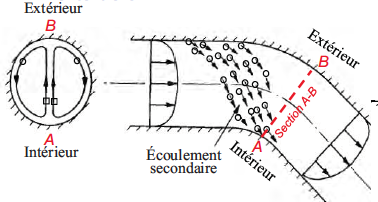
\includegraphics[scale=0.50]{ch6/82.png}
\caption*{Figure 6.20}
\end{center}
\end{figure}

De manière générale, un coude brusque présente plus de décollements, des décollements plus intenses et des écoulements secondaires plus intenses $ \rightarrow $ les pertes locales sont plus importantes ($ \zeta >> $) pour un coude brusque que pour un coude progressif. Cependant un coude progressif est plus encombrant.

Si le rayon de courbure relatif $R_0/D \uparrow$, le coude devient de plus en plus progressif (mais également de plus en plus encombrant).
\begin{itemize}
\item Dans un premier temps, les pertes locales diminuent car les décollements à l’intérieur et à l’extérieur du coude diminuent puis disparaissent et les écoulements secondaires diminuent.
\item Dans un second temps, si $R_0/D$ continue à augmenter, la longueur du coude augmente et les pertes par frottement sur les parois augmentent.
\end{itemize}
 $\rightarrow $ Pour un angle de coude $\alpha $ fixé, il existe un optimum pour les pertes locales en fonction du rayon de courbure relatif $R_0/D$ (cf. figure 6.21).
 
Dans le cas d’un coude à angle vif et du progressif, une façon simple d’éviter les décollements parasites est d’installer une série de lames cintrées ou d’aubages fixes. Les canaux entre les lames cintrées ayant une courbure relative plus faible :
\begin{itemize}
\item  Réduisent ou suppriment les décollements dans la partie extérieur ou intérieur du coude. Ceci a donc tendance à diminuer les pertes de charge singulières.
\item Réduisent l’intensité des écoulements secondaires et donc des pertes tourbillonnaires associées. Ceci a donc à également tendance diminuer les pertes de charge singulières.
\end{itemize}

Néanmoins, l’ajout de lames augmente la superficie des surfaces en contact avec le fluide et donc les frottements visqueux: Les pertes de charge par frottement ont donc tendance à augmenter avec le nombre de lames. En conséquence, pour diminuer le coefficient de perte singulier du coude, il existe un compromis entre un nombre suffisamment important de lames pour supprimer les décollements et limiter les pertes  econdaires par tourbillon et suffisamment faible pour ne pas augmenter de manière démesurée les pertes par frottement visqueux le long des parois des lames.

\begin{minipage}{0.49\textwidth}
\begin{figure}[H]
\begin{center}
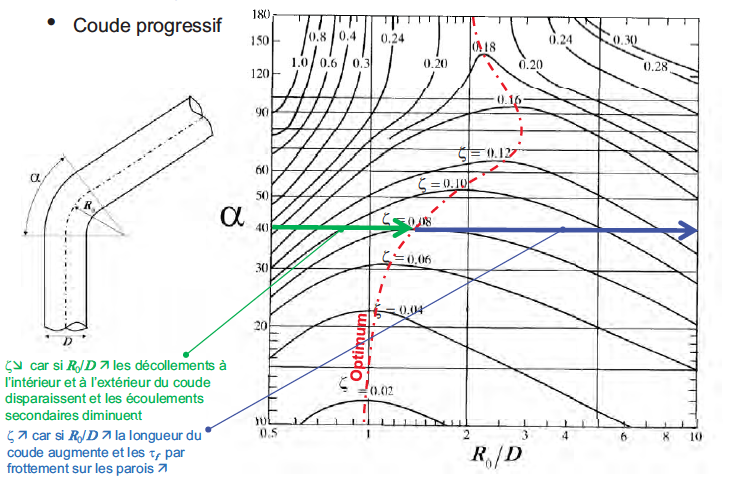
\includegraphics[scale=0.3]{ch6/83.png}
\caption*{Figure 6.10}
\end{center}
\end{figure}
\end{minipage}
\begin{minipage}{0.49\textwidth}
\begin{figure}[H]
\begin{center}
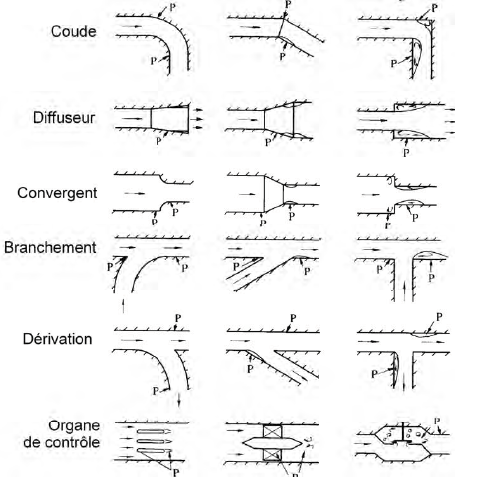
\includegraphics[scale=0.35]{ch6/84.png}
\caption*{Figure 6.11}
\end{center}
\end{figure}
\end{minipage}

\section{Pertes de charge singulières dans les branchements et les dérivations (Cours de Mons)}

Le Pr. Degrez a passé cette section mais je note quand mêmes quelques notes intéressantes.
\\

Notes:
\begin{itemize}
\item Dans les raccordements, il y a une variation de charge totale, combinaison de la perte de charge singulière proprement dite (variation négative de la charge) et de la variation de charge provoquée par la variation de débit (variation négative ou positive de la perte de charge).
\item Hypothèse de non-interaction des pertes des perturbations locales: La perte de charge globale est la somme des pertes de charges réparties et des pertes de charges locales.
\item Enfin la figure 6.23 reprend les formules globales pour les pertes de charges dans le cas rugueux et laminaire.
\\
\end{itemize}

\begin{figure}[H]
\begin{center}
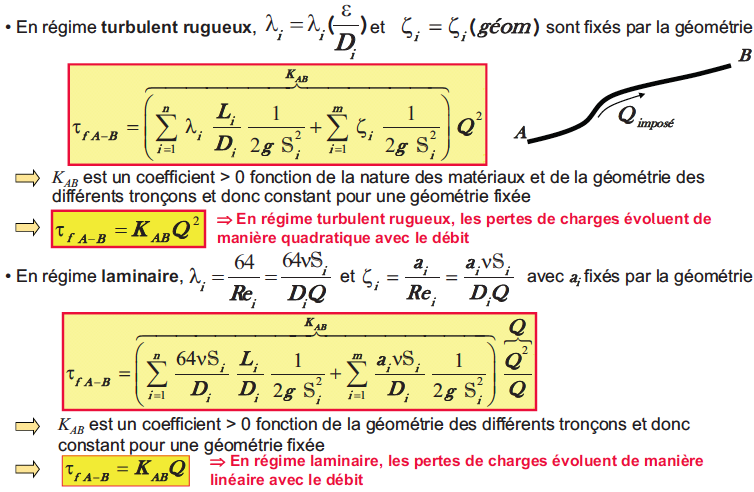
\includegraphics[scale=0.5]{ch6/85.png}
\caption*{Figure 6.23}
\end{center}
\end{figure}


\section{Problème de canalisations multiples en réseau (Cours de Mons)}

La figure ci-dessous reprend les deux résultats importants de ce court chapitre. A savoir, la loi des mailles et la loi des noeuds.

\begin{figure}[H]
\begin{center}
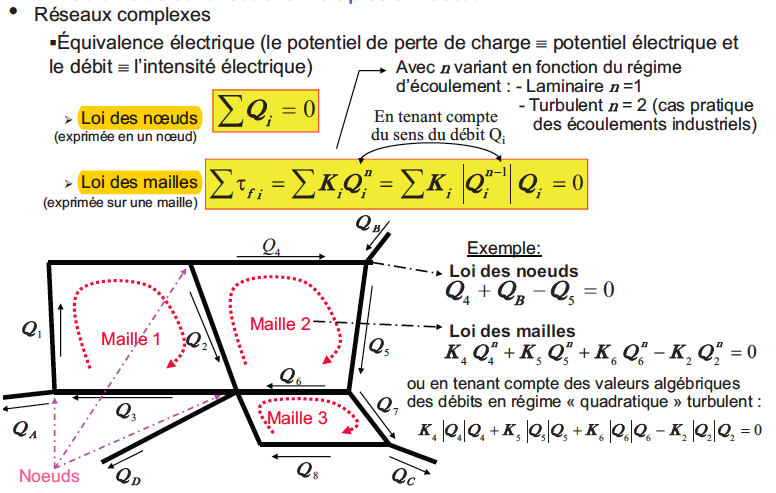
\includegraphics[scale=0.5]{ch6/86.png}
\caption*{Figure 6.24}
\end{center}
\end{figure}
